\section{eo\-Vector$<$ Fit\-T, Gene\-Type $>$ Class Template Reference}
\label{classeo_vector}\index{eoVector@{eoVector}}
Base class for fixed length chromosomes, just derives from {\bf EO}{\rm (p.\,\pageref{class_e_o})} and std::vector and redirects the smaller than operator to EO (fitness based comparison).  


{\tt \#include $<$eo\-Vector.h$>$}

Inheritance diagram for eo\-Vector$<$ Fit\-T, Gene\-Type $>$::\begin{figure}[H]
\begin{center}
\leavevmode
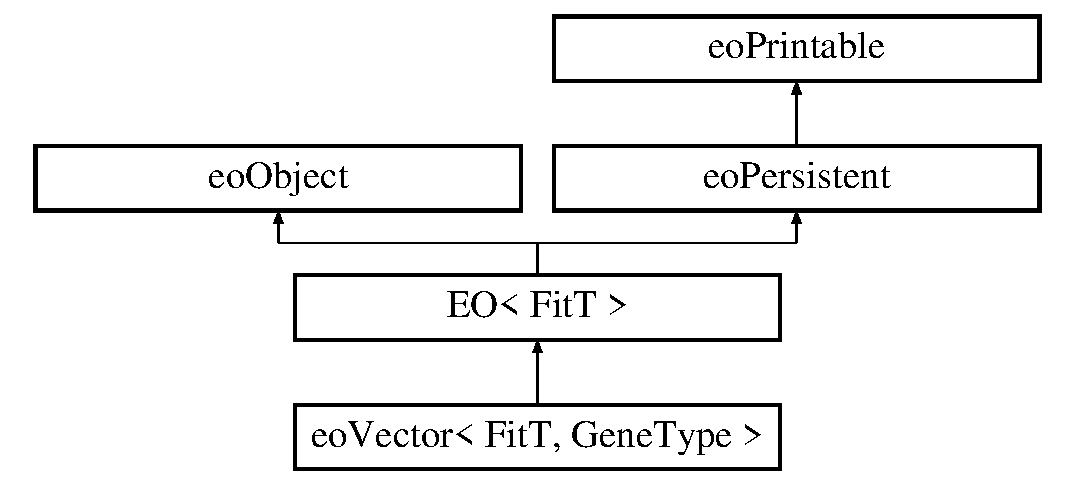
\includegraphics[height=4cm]{classeo_vector}
\end{center}
\end{figure}
\subsection*{Public Types}
\begin{CompactItemize}
\item 
typedef Gene\-Type {\bf Atom\-Type}\label{classeo_vector_w0}

\item 
typedef std::vector$<$ Gene\-Type $>$ {\bf Container\-Type}\label{classeo_vector_w1}

\end{CompactItemize}
\subsection*{Public Member Functions}
\begin{CompactItemize}
\item 
{\bf eo\-Vector} (unsigned size=0, Gene\-Type value=Gene\-Type())
\begin{CompactList}\small\item\em default constructor \item\end{CompactList}\item 
template$<$class Other\-Fitness\-Type$>$ {\bf eo\-Vector} (const {\bf eo\-Vector}$<$ Other\-Fitness\-Type, Gene\-Type $>$ \&\_\-vec)\label{classeo_vector_a1}

\begin{CompactList}\small\item\em copy ctor abstracting from the Fit\-T \item\end{CompactList}\item 
void {\bf value} (const std::vector$<$ Gene\-Type $>$ \&\_\-v)\label{classeo_vector_a2}

\item 
bool {\bf operator$<$} (const {\bf eo\-Vector}$<$ {\bf Fit\-T}, Gene\-Type $>$ \&\_\-eo) const \label{classeo_vector_a3}

\begin{CompactList}\small\item\em to avoid conflicts between EO::operator$<$ and std::vector$<$Gene\-Type$>$::operator$<$ \item\end{CompactList}\item 
virtual void {\bf print\-On} (std::ostream \&os) const \label{classeo_vector_a4}

\begin{CompactList}\small\item\em printing... \item\end{CompactList}\item 
virtual void {\bf read\-From} (std::istream \&is)\label{classeo_vector_a5}

\begin{CompactList}\small\item\em reading... \item\end{CompactList}\end{CompactItemize}


\subsection{Detailed Description}
\subsubsection*{template$<$class Fit\-T, class Gene\-Type$>$ class eo\-Vector$<$ Fit\-T, Gene\-Type $>$}

Base class for fixed length chromosomes, just derives from {\bf EO}{\rm (p.\,\pageref{class_e_o})} and std::vector and redirects the smaller than operator to EO (fitness based comparison). 

Gene\-Type must have the following methods: void ctor (needed for the std::vector$<$$>$), copy ctor, 



Definition at line 46 of file eo\-Vector.h.

\subsection{Constructor \& Destructor Documentation}
\index{eoVector@{eo\-Vector}!eoVector@{eoVector}}
\index{eoVector@{eoVector}!eoVector@{eo\-Vector}}
\subsubsection{\setlength{\rightskip}{0pt plus 5cm}template$<$class Fit\-T, class Gene\-Type$>$ {\bf eo\-Vector}$<$ {\bf Fit\-T}, Gene\-Type $>$::{\bf eo\-Vector} (unsigned {\em size} = {\tt 0}, Gene\-Type {\em value} = {\tt GeneType()})\hspace{0.3cm}{\tt  [inline]}}\label{classeo_vector_a0}


default constructor 

\begin{Desc}
\item[Parameters:]
\begin{description}
\item[{\em size}]Length of vector (default is 0) \item[{\em value}]Initial value of all elements (default is default value of type Gene\-Type) \end{description}
\end{Desc}


Definition at line 65 of file eo\-Vector.h.

The documentation for this class was generated from the following file:\begin{CompactItemize}
\item 
eo\-Vector.h\end{CompactItemize}
